\chapter{Implementation}
\label{sec:implementation}
% Hier greift man einige wenige, interessante Gesichtspunkte der
% Implementierung heraus. Das Kapitel darf nicht mit Dokumentation oder
% gar Programmkommentaren verwechselt werden. Es kann vorkommen, daß
% sehr viele Gesichtspunkte aufgegriffen werden müssen, ist aber nicht
% sehr häufig. Zweck dieses Kapitels ist einerseits, glaubhaft zu
% machen, daß man es bei der Arbeit nicht mit einem "Papiertiger"
% sondern einem real existierenden System zu tun hat. Es ist sicherlich
% auch ein sehr wichtiger Text für jemanden, der die Arbeit später
% fortsetzt. Der dritte Gesichtspunkt dabei ist, einem Leser einen etwas
% tieferen Einblick in die Technik zu geben, mit der man sich hier
% beschäftigt. Schöne Bespiele sind "War Stories", also Dinge mit denen
% man besonders zu kämpfen hatte, oder eine konkrete, beispielhafte
% Verfeinerung einer der in Kapitel 3 vorgestellten Ideen. Auch hier
% gilt, mehr als 20 Seiten liest keiner, aber das ist hierbei nicht so
% schlimm, weil man die Lektüre ja einfach abbrechen kann, ohne den
% Faden zu verlieren. Vollständige Quellprogramme haben in einer Arbeit
% nichts zu suchen, auch nicht im Anhang, sondern gehören auf Rechner,
% auf denen man sie sich ansehen kann.




% Also kurzer Überblick über die Struktur schreiben, dann auf GRPC eingehen. Wenn GRPC erklärt wurde, würde ich den DC_rounds Service vorstellen. Dann pseudoartig auf die Funktionen eingehen und ein Diagram zeichnen.
%Wo gab es probleme bei der implementation? Es gab probleme bei der synchronisation der unterschiedlichen teilnehmer.-> unterschiedliche Sekunden. Außerdem war es neu, dass mehrere nutzer auf den selben servercode "zugreifen" und das parallele programmieren. die fork nicht vergessen.
% wo gibt es unterschiede? design von grpc eingehen, man kann keine Nachrichten weiterleiten mit grpc. Nur 2 verbindungen zwischen CLients möglich.vllt noch mehr?
The conceptual approach of the DC network was presented in Chapter 3. Nevertheless, smart grids are a real-world system and it must be shown that the theoretical solution can be implemented in a practical environment. This chapter deals with the implementation of the introduced protocol. It is described which technical tools were used and at which implementation steps problems occurred.
\section{Structure of the practical implementation}
A DC network was implemented with the same requirements as defined in chapter 3. For technical reasons, however, the exact same structure could not be implemented. If there are any deviations from the defined protocol, then these will be described and explained in this chapter.
4 Raspberrypis are used to realise the design, where 3 Raspberrypis simulate the SMGW and 1 Raspberrypi represents the electricity provider.  In the following, the Raspberrpis that represent the SMGW are called clients and the Raspberrypi that represents the power provider is simply referred to as the power provider. All clients have a communication link via Lan to the power provider. However, the clients do not have a physical connection to each other. As suggested in the protocol, the only way for the clients to communicate is through the power provider. After the clients join the DC network, the clients build their local sum and send it periodically to the power provider. The electricity provider adds up the local totals and stores the global total in an external text file. In a smart grid, electricity consumption is sent to the electricity provider every 15-60 minutes. Since the implementation is a demo, the sending interval is 10 seconds. In addition, the demo was implemented in such a way that after 4 messages a client fails and a corrective action must be taken. After that the client can re-enter the DC network. To avoid having to implement the application and the related network protocol, gRPC was used as a framework.\\
\\
\textbf{gRPC Remote Procedure Calls - GRPC}
%hier ein kleiner text
\\
\\
GRPC is an open source remote procedure call (RPC) system developed by Google since 2015. GRPC relies on a client-server structure and simplifies the construction of linked systems. With GRPC, so-called services can be defined. Each service allows to declare different functions that can communicate via a self-selected message format referred to as Protocol Buffers. Therefore on the client the functions are implemented, while the server runs the interface and processes the client requests. On the client there is a stub that holds the same functions that are on the server. In gRPC server and client can communicate with each other, although they were implemented in different programming languages. In this work, both server and client were implemented in Python. A simple application example is shown in Figure 4.1.
\begin{figure}[tbp]
  \centering
  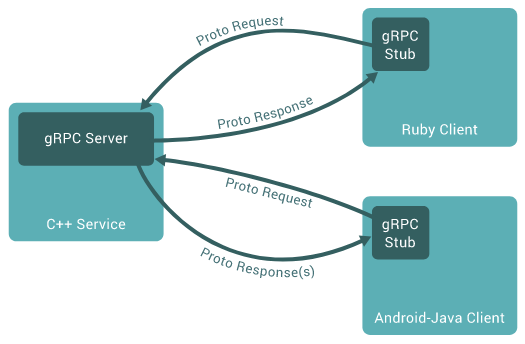
\includegraphics[width=0.8\textwidth]{images/grpc.png}
  \caption[gRPC Framework Structure]{An overview of the structure between client and server in gRPC.}
  \label{fig:Appliance_Model}
\end{figure}\\
\\
\textbf{Protocol Buffers in gRPC}
%hier ein kleiner text
\\
\\
Protocol buffers are used by default in gRPC and allow structured data to be serialized. With Protocol Buffers, structured data can be specified as message formats. Then the source code is automatically generated from the structured data and it can be sent through channels provided by e.g. gRPC.
Listing \ref{listing4.1} shows the implementation of the protocol header as a protocol buffer. Each header field is assigned a data type and also a unique field number that determines the order of the fields.\\
%\label{listing4.1} 
\lstinputlisting[language=protobuf2, style=protobuf,caption={%
The implementation of the DC network protocol header in a Protocol Buffer message format.}]{protobuf/dc_net.proto}
%\lstinputlisting[language=protobuf2, style=protobuf,caption={%
%The implementation of the DC network protocol header in a Protocol Buffer %message format.}]{protobuf/dc_net.proto}%\label{listing4.1}
\subsection{Server Implementation}
The server implements all functions that are defined as a service in the protocol buffer. The client implements most of the logic of the DC network. However, when the client accesses a service, most of the service functionality is implemented on the server. Therefore, the client prepares all necessary data and sends the data over a communication channel to the server. The data is then processed by the server and the result is communicated to the client as a response. Listing \ref{listing4.2} shows all service functions implemented on the server. %The data is then processed by the server and the result is communicated to the client as a response. Listing \ref{listing4.2} shows all service functions implemented on the server. 
Each function in the service is defined as an RPC and a name is assigned to the function. In addition, the RPC can accept a message format. For example, the addClientToDCnet function uses the message format defined in Listing \ref{listing4.1}. 
\\
%\label{listing4.2}
\lstinputlisting[language=protobuf2, style=protobuf,caption={%
All server functions provided by the DC network service to the client.}]{protobuf/dc_net_server.proto}
%\lstinputlisting[language=protobuf2, style=protobuf,caption={%
%All server functions provided by the DC network service to the client.]}{protobuf/dc_net_server.proto}
%\label{listing4.2}
\\ The functions of the service can be divided into 2 categories. First, helper functions for registration or initialization into the DC network. Second, functions in which logic of the DC net is implemented. In the following, the task of the helper functions is described first. Then the more complex functions are described, which also contain logic of the DC network.\\
\subsection{Client Implementation}
%hier ein kleiner text
When the in client application starts, a fork function is executed on client side. The fork function allows an process to create a second process by duplicating the address space of the calling process. The calling process is called parent and the duplicated process is called child. In the application, the parent process takes care of the child process. If the child process crashes, the parent process ensures that the child is restarted correctly. The main logic of the DC network is found in the child process of the client. Only in the child process the services provided by the server are called and used. In addition, the communication channel of gRPC is implemented only on the child. The communication channel forms the interface in which the defined protocol buffers can be sent as messages. This means that the parent process has no access to the communication between server and client. Once the communication channel is configured, the interaction between client and server can begin. Figure 4.2 illustrates the structure of the client implementation in a flow chart.
%In the demo, a client is periodically forced to crash so that the error correction procedures can be demonstrated. The actual logic of the application and the communication between client and server is located in the child process. 
\\
\\
\textbf{Initialization}
\\
\\
First, it is assumed that the server is already started. Otherwise, the client cannot be started in gRPC, since no communication channel can be created. The server waits for requests from the client and processes the requests. Second, the child establishes a connection to the electricity provider. In response, the child receives a DC Net identifier and a client identifier. A registering client is stored with Client Identifier by the server in a list. This gives the server an overview of the number of participants in the DC Net. In addition, the server can identify faster which client could not send its messages in case of error correction measures. \\
\\
\textbf{Registration}
\\
\\
After a client has received a DC Net identifier and a client identifier, the client requests the server to assign it a random neighbor. In order for the neighbor and the registering client to synchronize their PRNG, both have to perform a Diffie Hellman key exchange. All the necessary information for calculating the public key is provided by the server and is communicated to the clients on request. In the proposed protocol from the previous chapter, it was described that the electricity provider must offer a tunnel so that two SMGWs can communicate and exchange public keys via Diffie Hellman with each other. The tunnel in the protocol represents the communication channel in gRPC. But in gRPC all RPC requests are started by the client. The server only responds to the client's requests. Forwarding messages from a requesting Clients to a non-requesting clients is therefore not possible or very difficult to implement in gRPC. Instead of the public keys being forwarded to the clients by the server, as suggested in the protocol, the public keys are stored by the clients on the server for a short time and the clients make a request for the public keys. 
Each client only needs to obtain the public key of its neighbor through a request and is able to compute the secret key. After the Diffie Hellman key exchange has been executed and the PRNG has been configured, the client can create the local sum and send its local sum to the power provider/server for each round. 
\\
\\
\textbf{Generation of the global Superposition}
\\
\\
The server receives all the local sums and adds them up to get the global sum. Subsequently the server verifies the correctness of the global sum. If the global sum is incorrect, then a client in a DC network has failed and could not send a local sum. The defective client is located by the server by looking up which client has not sent a local sum to the server. Afterwards the neighboring clients are instructed by the server to recalculate the local sum without using the key of the failed client and resent it to the server. The global sum is then updated by the power provider. \\
\\
\textbf{Preparations for the next Round}
\\
\\
After each sending of the local sum, all clients check whether a new subscriber wants to register in the DC network. If so, one client is notified by the server that it gets a new neighbor. Then another registration process takes place with the Diffie Hellman key exchange which was described before. Then another registration process takes place with the Diffie Hellman key exchange which was described before. Another deviation from the protocol is that in the implementation each client has no minimum number of neighbors than the required 3 neighbors in the protocol. The flow chart in Figure \ref{fig:Client Implementation} illustrates the structure of the client implementation with the key functions.
\begin{figure}[tbp]
  \centering
  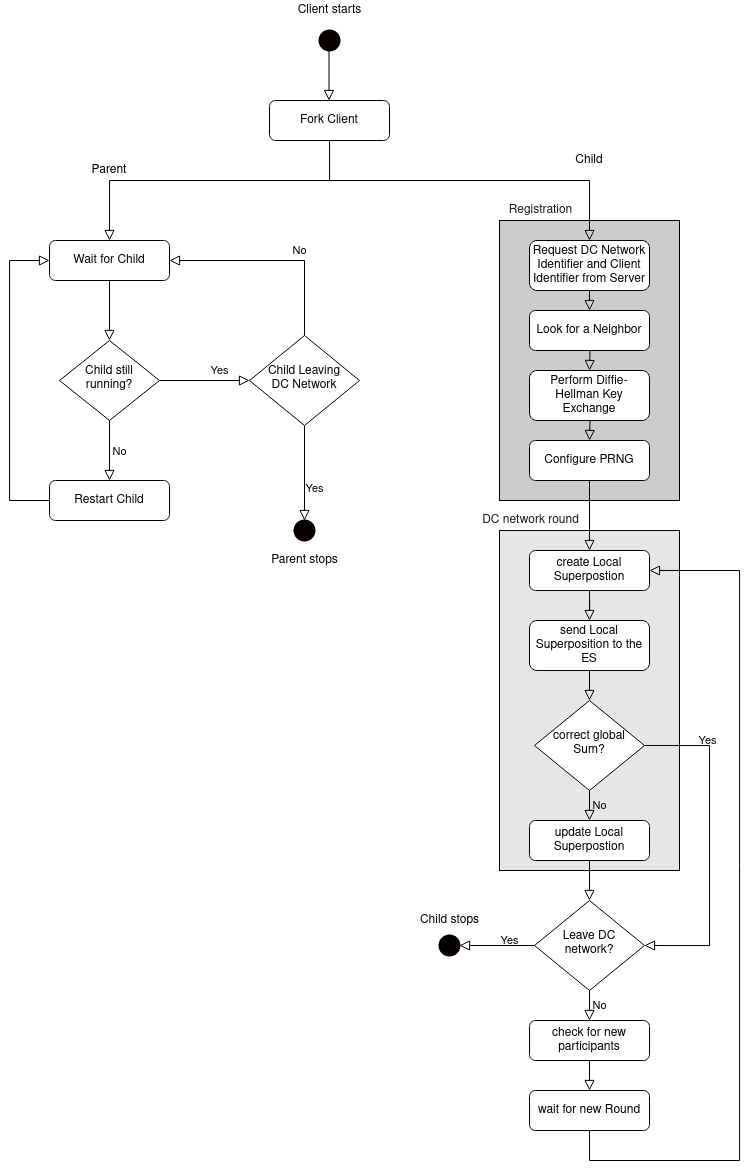
\includegraphics[width=0.8\textwidth]{images/Client_structure.png}
  \caption[Flowchart Client Implementatioen]{The flowchart shows all program operations that are performed in the client.}
  \label{fig:Client Implementation}
\end{figure}

%\\
%\textbf{Helper Functions}
%%\\
%\\
%The helper functions in the service mainly perform tasks to register the client in the DC network or to ensure client communication with each other. Therefore, the helper functions do not take over any core logic in the DC network. In the following a documentation with the tasks of the functions is described.
%\begin{enumerate}
%\item addClientToDCnet:\\
%The first action that the client child performs is to register on the DC network. For this the addClientToDCnet function is used. In the server the request from the client is processed. The client is assigned a client identifier and the identifier is added to a list so that the service has an overview of all clients in the DC network.
%\item ConnectDCClients:\\
%The ConnectDCClients function assigns a random neighbor to a requesting client.

%\end{enumerate}
%\\
%\\
%\textbf{DC Network Functions}
%\\
%\\

\section{Challenges}
Several challenges were encountered during the implementation in this thesis. The most serious and time-consuming 3 errors are described below.\\
\\
\textbf{Multiple Client access on the Server}
\\
\\ 
In the experimental environment, 3 clients communicate with a server. A particular challenge was therefore to implement the server cleanly and consistently so that multiple clients could access the same function or even the same line of code  at the same time without the server crashing or the program entering an inconsistent state. The implementation was therefore particularly difficult in the service functions in which the calculations of the global sum or the verification of the global sum was carried out.%vllt noch irgendwas schreiben mit Da der Author zuvor noch keine Erfahrung in verteilen Programmieren hatte etc.
\\
\\
\textbf{gRPC Client-to-Client Communication}
\\
\\
The protocol defined that the electricity provider must provide a tunnel for SMGW to SMGW communication. It was tried to implement the same structure as in the protocol. However, the clients in the gRPC framework do not receive an IP address, so the server cannot distinguish calls from different clients. In search of a solution the following suggestions have been considered. 
\begin{enumerate}
\item Setup a Server on each Client:\\
In this approach, each RaspberryPi on which a client application is implemented would get an additional server that can communicate with the power provider. In addition, a client would have to be implemented on the power provider so that requests from the power provider can be sent to clients over a communication channel. In the work it was decided against it, because it is a considerable additional effort and requires an extra implementation of servers on the clients.
\item Bi-directional Streaming:\\
gRPC offers different ways to send messages. One way is a bidirectional streaming RPC where server and client exchange a sequence of messages. In gRPC both streams work independently and can be configured depending on the use.%den satz überarbeiten
In a message stream the server can wait for all client requests before responding or it can respond immediately after each message.  A stream can be defined in the Protocol Buffer syntax with the keyword stream. The stream property can be exploited to implement message forwarding in gRPC. Various solution sketches have been found that promote this approach. However, the proposed solutions were vague and storing the public keys in the short term on the server was much simpler to implement. 

\end{enumerate}\\
\\
\textbf{Crashing Parent}
\\
\\
During the implementation there were indeterministic crashes of the parent in the client. The error could not be traced for a long time, because the crash occurred at different times during the runtime of the application. When the parent crashes, the child continues to work without interruptions. However, the child cannot be restarted if the parent crashes. It has been found by accident that the fork function is not executed correctly after the communication channel has been created.  
%sowas schreiben wie, dass der Mehrfachzugriff auf den Server problematisch war und schwer zu implementieren, da du noch nie mit verteilten Systemen gearbeitet hast. Dann noch schreiben, dass grpc die technischen mögichkeiten eingeschränkt hat, da es keine Client zu CLient kommunikation gab. Vllt zusammenfassen, dass die Clients einfach zu implementieren waren, aber die schwerste aufgabe der server war. Das Problem mit dem Kommunikationskanal und das der Parent die ganze zeit abgestürzt ist.

%Den Service noch beschreiben!

%%% Local Variables:
%%% TeX-master: "diplom"
%%% End:

\cleardoublepage